The Logipedia consortium will gather twenty-eight beneficiaries and partners
from eleven European countries for four years. The project management
structure will be tailored to the specificities and needs of this
large consortium and its ongoing network development.

%%%%%%%%%%%%%%%%%%%%%%%%%%%%%%%%%%%%%%%%%%%%%%%%%%%%%%%%%%%%%%%%%%%%%%%%%%%%%%
\subsection*{Organisational structure}

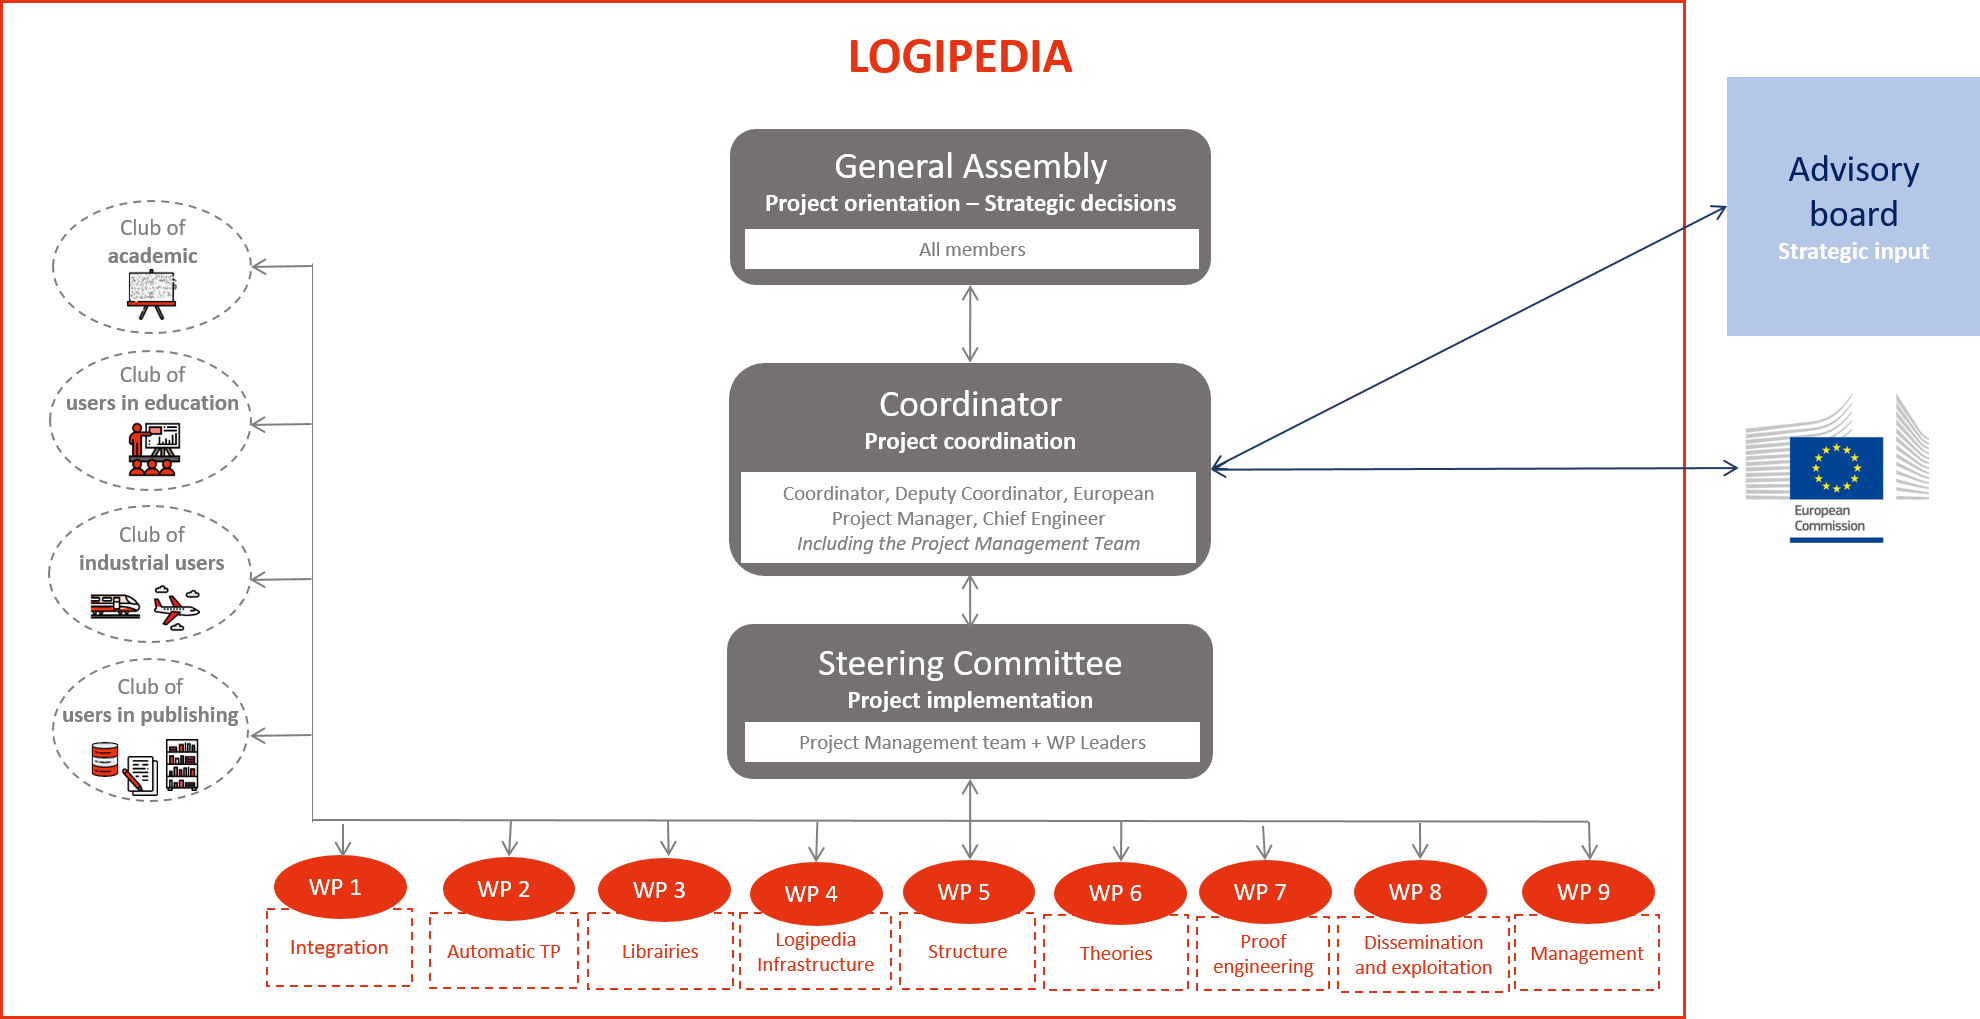
\includegraphics[width=\textwidth]{img/Gouvernance}

\subsubsection*{The project management team}

\begin{compactitem}
\item{\bf The Coordinator} is responsible for the coordination of
scientific and technical activities in order to meet the objectives
set by the European Commission in the Grant Agreement. The 
coordinator works closely with the work package leaders
within the steering committee, in order to monitor the progress of the
scientific and technical work and identify potential risks within each
work package. The coordinator will daily
collaborate with the European project manager in charge of the
day-to-day management of Logipedia. The project will be managed by
Gilles Dowek, permanent senior researcher at Inria Saclay. He will
also chair the meetings of both the general assembly and steering
committee.

\item{\bf The Deputy Coordinator} seconds the coordinator.

\item{\bf The European Project Manager} 
  is a team member of the Technology Transfer and Partnership Office
  of Inria Saclay. He or she is in charge of all administrative,
  financial and legal management tasks as listed in
  \WPref{management}. The European project manager is the interface
  between the project and the European Commission as it represents the
  point of contact for the European Commission. The European project
  manager has the overall administrative and financial responsibility
  for the organisation and administrative and financial monitoring of
  the project.

\item{\bf The Chief Engineer} is an experienced
research engineer from Inria Saclay and is responsible for ensuring
the development and maintenance of tools at Inria Saclay and
supervising the development tasks achieved at the other
beneficiaries. The chief engineer will ensure the coherence of the
Logipedia tools development, according to the defined schedule in the
Grant Agreement.
\end{compactitem}

Innovation management and intellectual property rights issues will be
handled by the European project manager, supported by the experienced
Technology Transfer and Partnerships Office of Inria Saclay. The
project management team will establish appropriate policies and rules
for the management of intellectual property rights for the knowledge
developed within the project, as well as the identification of the
opportunities for the exploitation of the project results in
innovation activities. Issues related to innovation and/or
intellectual property rights management will be tackled at every
steering committee meeting.

\subsubsection*{The operational level}

\begin{compactitem}
\item{\bf The Steering Committee}:
The steering committee is composed of the Coordinator, the Deputy
coordinator, the Chief engineer, the European project manager and the
work package leaders.  It is the main decision-making body of the
project. It coordinates activities within and among the workpackages,
evaluates and validates the progress of the project, assists the
scientific coordinator in carrying out his tasks, monitors the
technical direction of the project, approves all major technical
decisions, approves all deliverables, approves all significant changes
in the project work plan, reviews and amends the work plan. The
Steering Committee is responsible for the implementation of decisions
made by the general assembly. It can formulate proposal for changes in
the description of action and the related consortium budget. The
steering committee is chaired by the coordinator.

\item{\bf The Work Package Leaders}: The work package leaders are
responsible for the monitoring and management of the activities and
results within their work packages. In particular, work package
leaders i) identify deviations from the project plan and report them
to the steering committee, ii) manage and supervise the preparation of
reports and their timely delivery, iii) control and monitor activities
of tasks and regularly meet once per month with task leaders, iv)
manage the information flow with other work packages via the steering
committee.

\item{\bf The Task Leaders}: The task leaders are responsible for
coordinating the scientific and technical work in their task and
making the day to day technical decisions that solely affect their
task. Inter-task decisions are coordinated with the work package
leaders.

\item{\bf The Club Leaders}: The club leaders are in charge of
  disseminating of the results and tools developed by the Logipedia
  consortium in various communities. They organise the activity of the
  club. They give ongoing feedback to the consortium during the course
  of the project.
\end{compactitem}

\subsubsection*{The strategic level}

\begin{compactitem}
\item{\bf The General Assembly}: The general assembly is composed by all
the members of the consortium, with each representative having one
vote. Every new partner will have a voting right. The general assembly
will gather at least once a year, and as many virtual meetings as
needed. The general assembly is the main governance and ultimate
decision-making body of the consortium. The general assembly must
review the project progress, decide on contingency actions in case of
deviations from the plan and take final decisions on policy and
contractual issues and conflicts as requested by the steering
committee.

\item{\bf The Advisory Board}: The advisory board is a consultation body to
the steering committee and general assembly. It will bring external
and non-legally binding perspective on the scientific and technical
development of the project, ecosystem building and the future of the
encyclopedia. The advisors of this board will attend the yearly
general assembly plenary meeting and will be consulted on the strategy
of the project. The advisory board should aim at representing the
stakeholders of the Logipedia ecosystem without including any
beneficiary or associate partner’s employees. It will be composed of,
among others, industrial and international academic partners
(including non-European ones) appointed by the coordinator after
consulting the steering committee. To start with, we suggest to
include: June Andronick (Data61, Kensington NSW, AU), Denis Cousineau
(Mitsubishi Electric R\&D Centre Europe, FR), Thomas Letan (ANSSI, FR),
Jacques Fleuriot (University of Edinburgh, UK), Natarajan Shankar
(SRI, US), Aaron Stump (Iowa University, US), Laurent Voisin
(Systerel, FR).
\end{compactitem}

\subsubsection*{Internal communication and collaborative ecosystem}

The consortium will make use of a number of
project management tools, such as a visio conferencing tool, a project
repository to have an updated account of the project’s important
documents, the progress of the work packages work and deliverables,
all the advances in the project and all the meetings minutes, mailing
lists, etc. that facilitate the smooth execution of the project. This
collaboration environment will be provided by the coordinator of the
project.

Work packages, chaired by work package leaders, will have monthly
planned visio conferences and meetings as need by the work plan.
Additional technical meetings may be set up by task leaders or
individual partners. The steering committee will have monthly visio
conferences and will meet twice a year. Dedicated working groups will
be planned as needed according to the work plan.  All meetings will be
documented by minutes listing major decisions and action items.

The project management team will be in charge of all organisational
issues in the general assembly meetings, supported by the local
partner. The project will organise meetings of the general assembly at
least once a year. To equally share travel costs among partners,
physical meetings will be located by rotation at partners’
locations. Project review meetings will be done on a regular basis
according the Grant Agreement provisions.


%%%%%%%%%%%%%%%%%%%%%%%%%%%%%%%%%%%%%%%%%%%%%%%%%%%%%%%%%%%%%%%%%%%%%%%%%%%%%%

\subsection*{Quality Control}

Quality Control will be part of the
Logipedia Quality Plan, which will be a deliverable.

These guidelines adopted by Logipedia will ensure that all
participants know who, how and when to act regarding to documentation
of project activities, periodic reporting, preparation of financial
statements, approval and submission of deliverables, and risk
management.

The implementation of the quality management will include the following phases:
\begin{compactitem}
  \item 
identification of the procedures needed,
\item
planning, design and development of the procedures and the forms to be implemented,
\item development of an implementation guide for all the partners.
\end{compactitem}

Quality assurance is the joint responsibility of all partners and will
be applied at all levels of the project’s activities. The goal is to
ensure the detection of mistakes and deviations in the project’s life
cycle as early as possible in order to apply the necessary corrective
actions or contingency plans systematically. Every contractual
deliverable, prior to its submission to the Commission, will be the
subject of a peer review by two persons not directly involved in
either the subject matter or the creation of that deliverable.
The coordinator will make a final check of the deliverable for
consistency and readability.



%%%%%%%%%%%%%%%%%%%%%%%%%%%%%%%%%%%%%%%%%%%%%%%%%%%%%%%%%%%%%%%%%%%%%%%%%%%%%%
\subsection*{Decision-making Process}

Our approach for the decision-making process is to locate the decision
as close as possible to the level responsible for the execution (from
task to general assembly level). Decisions are managed within
frequent project meetings, either on-site or via
teleconference. Decisions can be also managed by consultation. If
voting is needed, the agenda should clearly indicate this fact. Quorum
and voting rules will be defined in the Consortium
Agreement. Decisions are binding once the relevant part of the meeting
minutes has been accepted. Any changes to the project plan and scope
must be reviewed and approved by all levels of project management,
before proposing these changes to the steering committee and any
modifications will be considered rejected, after rejection on any of
these involved levels.

Another guiding principle is to avoid conflicts. Nevertheless, should
one arise, a conflict resolution will be ready to be put in place to
deal with it accordingly. The conflict resolution foresees that each
conflict will be mediated, solved or decided at the lowest level
possible. Attempts to solve issues within the consortium will be
carried out in increasing order of authority first at task level
(management of task leader), work package level (management of work
package leaders), and then following the management bodies till the
general assembly.

Before the Logipedia project starts, the consortium partners will sign
a Consortium Agreement wherein roles, responsibilities and mutual
rights and obligations will be defined. It will be in complete
accordance with the rules of the Grant Agreement and will adopt
the recommended guidelines laid down by the European Commission.

%%%%%%%%%%%%%%%%%%%%%%%%%%%%%%%%%%%%%%%%%%%%%%%%%%%%%%%%%%%%%%%%%%%%%%%%%%%%%%
\subsection*{Monitoring and reporting}

\subsubsection*{Internal reporting}

The project management team continuously monitors the project plan
with its milestones. Each work package leader will be
responsible for the correct execution of the implementation plan for
the corresponding work package. In terms of reporting, this means the work package leaders
will be in charge of gathering the information related to their own
work packages.

Regular audio-conferences of the Steering Committee are foreseen,
which allows work package leaders to identify risks and
discuss them together. This ensures that management (coordination,
European project manager) is aware of potential problems and
deviations and can initiate countermeasures long before a situation
becomes critical. This ensures to spot the blocking points and implements
the solution at the right time.

The following project meetings are planned:

\begin{compactitem}
\item one kick-off meeting at the beginning of the project, 
\item one Steering Committee meeting every two months,
\item one physical Steering Committee meeting every six months
  (reporting on work progress), which will be hosted by each work package 
  leader. We will couple these meetings with other ones so to reduce
  travels,
\item optional WP meetings whenever needed, 
\item four project meetings are planned, jointly with a General Assembly,
  Advisory Board, Steering Committee and the four Clubs meetings.
\end{compactitem}

The kick-off meeting will serve to launch the project, create a
benevolent, trustful, and encouraging atmosphere and adjust
expectations.

\subsubsection*{Reporting to the European Commission}

The Logipedia consortium will follow the mandatory reporting period
required by the European Commission. 

The project management team will provide the necessary templates in
order to achieve the reporting in due time. Work package leaders will
be asked to gather the relevant information provided by the task
leader regarding their work package and to summarise in order to be
reviewed by the steering committee. It will then be treated by the
coordinator and European project manager and sent to the
European Commission.

%%%%%%%%%%%%%%%%%%%%%%%%%%%%%%%%%%%%%%%%%%%%%%%%%%%%%%%%%%%%%%%%%%%%%%%%%%%%%%
\subsection*{Significant risks and associated contingency plans}
\label{sec:risks}

\subsubsection*{Scientific risks}

\begin{longtable*}{|p{0.30\textwidth}|p{0.10\textwidth}|p{0.50\textwidth}|}
\hline
{\bf Description of the risk}
&
{\bf Work packages involved}
&
{\bf Proposed measure of mitigation}
\\
\hline
We do not succeed to express some theories in Dedukti.
(Probability: medium. Severity: low.)

&
WP6
&
We have carefully divided the systems into two groups: those that do not
present risks (WP1) and those that do (WP6). The success we got with the
theories implemented in systems of the first group gives us confidence
that the theories implemented in those of the second can also be
expressed in Dedukti.  If one of them happens to be more difficult, we
can still build a large encyclopedia with the systems of the first
group. We can also extend Dedukti so that it can express more theories,
as we have already done in the past.
\\
\hline
Some libraries require too much time and memory
to be expressed in Dedukti (Probability: medium. Severity: low.)
&
WP3
&
There are several ways to mitigate this risk: optimise the
representation of data (sharing, elimination of redundancies, etc.), 
use faster and larger computers. This may also mean that some tasks
of this work package are premature and that we have to wait for
faster computers, that Moore's law will provide.
\\
\hline
No adoption from the community. (Probability: low. Severity: high.)
&
All 
&
The community may fail to adopt Logipedia for several reasons. Because
of a problem of design of Logipedia, in which case we will have to
understand what needs to be changed in a second version.  It may be
because the Logipedia community is too small.  This explains that we
have decided to include twenty-eight partners in the project.  It may
also be because of an insufficient dissemination activity.  This is
why we propose to create the four clubs of users and we will devote
time and energy to the animation of these clubs, together with other
dissemination activities, such as summer schools and conferences.
\\
\hline
\end{longtable*}

\pagebreak
\subsubsection*{Management risks}

\begin{longtable*}{|p{0.30\textwidth}|p{0.10\textwidth}|p{0.50\textwidth}|}
\hline
Brexit disrupts the project (Probability: low. Severity: medium.)
&
All (specially WP6, WP7)
&
As we have two partners from the United Kingdom, Brexit could be a risk
for our project. Yet, we are quite confident
that scientific
cooperation will continue after Brexit and that the British partners
of the project will continue to be part of it.
As this project is submitted during H2020 and nothing changes until
the end of 2020, Logipedia is safe for the start of the project. From
2021 onwards, we can hope some agreement will be concluded as the UK
already made public its willingness to maintain collaborations.
If it were not the
case, we would have to reallocate the impacted tasks to other partners. 
\\
\hline
One partner leaves (Probability: low. Severity: depends on the partner.)
&
All
&
The impact of such a default of one partner of course depends on the
partner. But, during the preparation of this project, we have been
careful to develop an atmosphere of trust and solidarity between the
partners. If this happened
we would need to adapt the objectives of the work package the partner
was supposed to contribute to.
\\
\hline
Difficulty to find people (doctoral students, post-docs, engineers, etc.)
(Probability: medium. Severity: low.)
&
All
&
This project will require hiring a fair number of people. This may be
difficult in some European countries. If this happens we will use the
size of the network to find candidates in other countries to meet
the objectives of the project.\\
\hline
\end{longtable*}

%%%%%%%%%%%%%%%%%%%%%%%%%%%%%%%%%%%%%%%%%%%%%%%%%%%%%%%%%%%%%%%%%%%%%%%%%%%%%%
\subsection*{Milestones}\label{sec:milestones}

As show by the Pert diagram above, two work packages, are critical, as
many others depend on them: work package 4 ``Access to the
encyclopedia'' that is focused on the development of the
infrastructure itself and work package 1 ``Integration'' that focuses
on populating this infrastructure with theories and proofs. All work
packages depend on work package 4, and work packages 3 ``Large
libraries'', work package 5 ``Structure of the encyclopedia'', and
work package 7 ``Proof engineering'' depend on work package 1.  As a
consequence five of our milestones are completions of the key tasks of
work packages 4 and 1.  No milestone is the completion of a task of
the two, more risky, joint research activity work packages: work
package 6 ``Theories'' and work package 7 ``Proof engineering'', which
is a sign of robustness of the project.
  

%\begin{longtable*}{|p{0.1\textwidth}|p{0.55\textwidth}|p{0.2\textwidth}|p{0.1\textwidth}|}
%%%%%%%%%%%%%%%%%%%%%%%%%%%%%%%%%%%%%%%%%%%%%%%%%%%%%%%%%%%%%%%%%%%%%%%%%%%%%%
%\hline
%1
%&
%Prototype version of Logipedia platform
%&
%deliverable D4.7
%&
%M 14
%\\
%\hline
%2
%&
%Opam for Logipedia
%&
%deliverable D4.3
%&
%M 20
%\\
%\hline
%\end{longtable*}

%\begin{longtable*}{|p{0.1\textwidth}|p{0.55\textwidth}|p{0.2\textwidth}|p{0.1\textwidth}|}
%%%%%%%%%%%%%%%%%%%%%%%%%%%%%%%%%%%%%%%%%%%%%%%%%%%%%%%%%%%%%%%%%%%%%%%%%%%%%%
%\hline
%3
%&
%Instrumentation of Isabelle 
%&
%deliverable D1.2
%&
%M 12
%\\
%\hline
%4
%&
%Instrumentation of HOL4 
%&
%deliverable D1.3
%&
%M 12
%\\
%\hline
%5
%&
%Instrumentation of Coq 
%&
%deliverable D1.6
%&
%M 8
%\\
%\hline
%\end{longtable*}

\begin{milestones}
\milestone[id=coq,verif=Inspection,month=8]
   {Instrumentation of Coq.}
   {Integration of the Coq standard library in Logipedia.}
\milestone[id=isabelle,verif=Inspection,month=12]
   {Instrumentation of Isabelle.}
   {Integration of the Isabelle standard library in Logipedia.}
\milestone[id=hol4,verif=Inspection,month=12]
   {Instrumentation of HOL4.}
   {Integration of the HOL4 standard library in Logipedia.}
\milestone[id=opam,verif=Inspection,month=12]
   {Opam for Logipedia.}
   {Release of a package distribution system for Logipedia.}
\milestone[id=platform,verif=Inspection,month=18]
  {Logipedia platform.}
  {Release of the web interface to the Logipedia platform.}
\milestone[id=evaluation,verif=Inspection,month=36]
   {First overall evaluation of the project.}
   {The delivery of the reports of the clubs of users allow to define
     the strategy for the long term exploitation of Logipedia.}
\end{milestones}

%%% Local Variables:
%%%   mode: latex
%%%   mode: flyspell
%%%   ispell-local-dictionary: "british"
%%% End:
